Vi har valgt at analysere vores project i forhold bohms model, samt at lave risici analyse p� forskellige muligheder mht. teknologi heriblandt: Android og Windows mobile, eventuelt kunne vi ogs� have overvejet mobile web. For hver enkelt teknologi skal overvejes specielt i forhold vores erfaring med den, samt relevans ift. m�let. \\

\subsection*{Bohms model}
% efterf�lgende skal opdateres
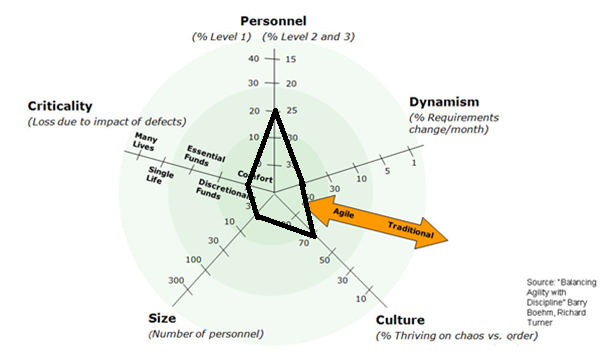
\includegraphics[scale=0.50]{includes/billeder/bohmsmodel.png}
I forhold til Bohms model er vi en MEGET lille gruppe, som drives p� chaos og personlig frihed. Samtidigt m� vi forvente at der bliver brug for meget dynamik idet at vi har s� lidt kendskab til teknologierne.

\begin{center}
\line(1,0){450}
\end{center}

\subsection*{Risici analyse}
\subsubsection*{Android mobile}
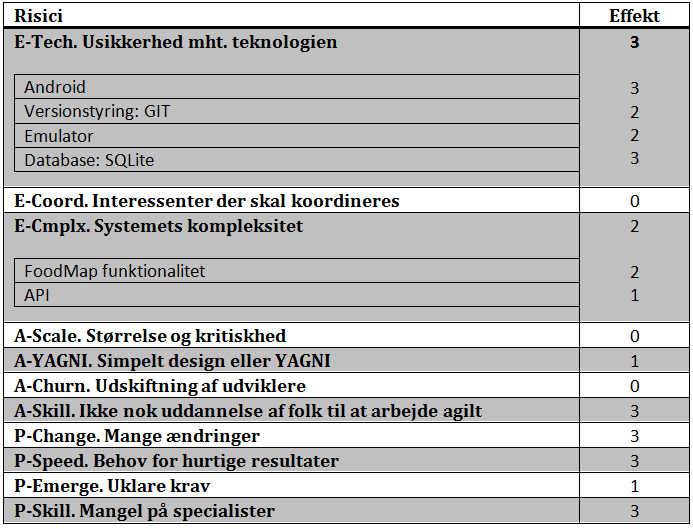
\includegraphics[scale=0.70]{includes/billeder/risici_analyse_android.png}

%\begin{itemize}
%\item E-Tech. Usikkerhed mht. teknologien: 2 
%\begin{itemize}
%\item Android ide: 2
%\item Versionstyring: 3
%\item Emulator: 1
%\end{itemize}
%
%\item E-Coord. Interessenter der skal koordineres: 0
%\item E-Cmplx. Systemets kompleksitet: 2
%\begin{itemize}
%\item FoodMap funktionalitet: 2
%\item API: 1
%\end{itemize}
%
%\item A-Scale. St�rrelse og kritiskhed: 0
%\item A-YAGNI. Simpelt design eller YAGNI: 1
%\item A-Churn. Udskiftning af udviklere: 0
%\item A-Skill. Ikke nok uddannelse af folk til at arbejde agilt: 3
%\item P-Change. Mange �ndringer: 1
%\item P-Speed. Behov for hurtige resultater: 2
%\item P-Emerge. Uklare krav: 1
%\item P-Skill. Mangel p� specialister: 3
%\end{itemize}

\begin{center}
\line(1,0){450}
\end{center}

\subsubsection*{Windows mobile} 
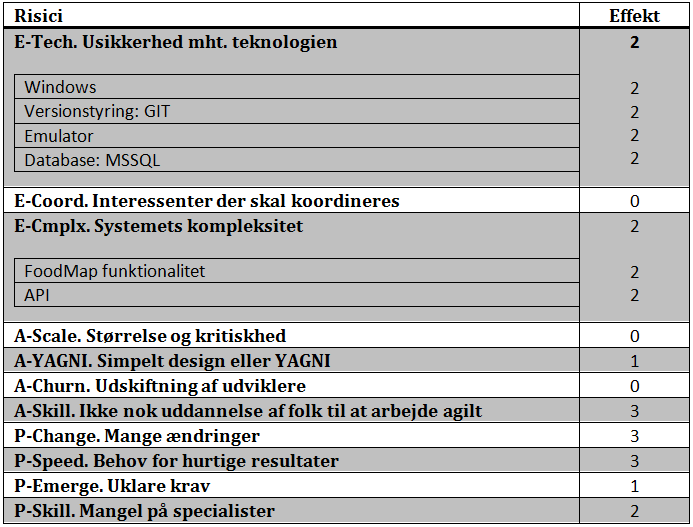
\includegraphics[scale=0.70]{includes/billeder/risici_analyse_windowsphone.png}
%\begin{itemize}
%\item E-Tech. Usikkerhed mht teknologien: 1
%\item E-Coord. Interessenter der skal koordineres: 1
%\item E-Cmplx. Systemets kompleksitet: 0
%\item A-Scale. St�rrelse og kritiskhed: 0
%\item A-YAGNI. Simpelt design elller YAGNI: 4
%\item A-Churn. Udskiftning af udviklere: 0
%\item A-Skill. Ikke nok uddannelse af folk til at arbejde agilt: 3
%\item P-Change. Mange �ndringer: 0
%\item P-Speed. Behov for hurtige resultater: 1
%\item P-Emerge. Uklare krav: 1
%\item P-Skill. Mangel p� specialister: 3
%\end{itemize}

\begin{center}
\line(1,0){450}
\end{center}

\subsection*{Metodevalg}
Begrundelse for metodevalg... \\
Vi er et sm�t hold som har det bedst med at der ikke er for stram en process. Specielt simpelt design er foretrukket... \\
Umiddelbart ud fra vores analyse ser det jo ud som om at Windows mobile er nemmere at tilg�, men idet at vi finder Android markedet mere relevant har vi valgt at arbejde med det.